\documentclass[11pt]{article}
\usepackage{homework}

\classname{443}
\homeworknum{3}



\begin{document}

% Environments

\newcommand{\state}[2]{\begin{statement}{#1} #2 \end{statement}}
\newcommand{\prob}[2]{\begin{problem}{#1} #2 \end{problem}}
\newcommand{\subprob}[1]{\begin{subproblem} #1 \end{subproblem}}
\newcommand{\sol}[1]{\begin{solution} #1 \end{solution}}
\newcommand{\fig}[2]{\begin{figure} \centering #2  \label{#1} \end{figure}}

\newcommand{\makebib}{
	\vfill
	\color{black}
	\nocite{*}
	\bibliography{references}{}
	\bibliographystyle{lucas_unsrt}
}
	

% Implication

\newcommand{\qwhere}{\quad \text{where} \quad}
\newcommand{\qimplies}{\quad \implies \quad}
\newcommand{\impliesq}{\implies \quad}



% Brackets

\newcommand{\paren}[1]{\left( #1 \right)}
\newcommand{\brac}[1]{\left[ #1 \right]}
\newcommand{\curly}[1]{\left\{ #1 \right\}}


% Greek

\newcommand{\alp}{\alpha}
\newcommand{\bet}{\beta}
\newcommand{\gam}{\gamma}
\newcommand{\del}{\delta}
\newcommand{\eps}{\epsilon}
\newcommand{\zet}{\zeta}
\newcommand{\tht}{\theta}
\newcommand{\kap}{\kappa}
\newcommand{\lam}{\lambda}
\newcommand{\sig}{\sigma}
\newcommand{\ups}{\upsilon}
\newcommand{\omg}{\omega}

\newcommand{\Gam}{\Gamma}
\newcommand{\Del}{\Delta}
\newcommand{\Tht}{\Theta}
\newcommand{\Lam}{\Lambda}
\newcommand{\Sig}{\Sigma}
\newcommand{\Omg}{\Omega}


% Text

\newcommand{\where}{\text{where }}

% Problem 1

\newcommand{\Hint}{H_\text{int}}
\newcommand{\ddcx}{\dd[3]{x}}
\newcommand{\psib}{\bar{\psi}}

\newcommand{\mh}{m_h}
\newcommand{\mmu}{m_\mu}
\newcommand{\me}{m_e}
\newcommand{\ma}{m_a}

\newcommand{\aexpt}{a_\text{expt.}}
\newcommand{\aQED}{a_\text{QED}}
\renewcommand{\GeV}{\giga\electronvolt}

\newcommand{\gamt}{\gam^5}


\state{Supersymmetry (Peskin \& Schroeder 3.5)}{
	It is possible to write field theories with continuous symmetries linking fermions and bosons; such transformations are called \emph{supersymmetries}.
}

\prob{}{	\label{3.5a}
	The simplest example of a supersymmetric field theory is the theory of a free complex boson and a free Weyl fermion, written in the form
	\eq{
		\cL = \ptsm \phis \ptm \phi + \chidag i \sigb \cdot \pt \chi + \Fs F.
	}
	Here $F$ is an auxiliary complex scalar field whose field equation is $F = 0$.  Show that this Lagrangian is invariant (up to a total divergence) under the infinitesimal transformation
	\aln{ \label{given1a}
		\del\phi & = -i \epsT \sigw \chi, &
		\del\chi &= \eps F + \sig \cdot \pt\phi \sigw \epss, &
		\del F &= -i \epsdag \sigb \cdot \pt\chi,
	}
	where the parameter $\epsa$ is a 2-component spinor of Grassmann numbers.
}

\sol{
	Using the supplied transformations and dropping terms of $\order{\del^2}$, we have
	\aln{
		\cL &\to \ptsm (\phis + \del\phis) \ptm (\phi + \del\phi) + (\chidag + \del\chidag) i \sigb \cdot \pt (\chi + \del\chi) + (\Fs \del\Fs) (F + \del F) \notag \\
		&\approx \ptsm \phis \ptm \phi + \ptsm \phis \ptm \del\phi + \ptsm \del\phis \ptm \phi + \chidag i \sigb \cdot \pt \chi + \chidag \sigb \cdot \pt \del\chi + \del\chidag i \sigb \cdot \pt \chi + \Fs F + \Fs \del F + \del \Fs F \notag \\
		&= \cL + \ptsm \phis \ptm \del\phi + \ptsm \del\phis \ptm \phi + \chidag \sigb \cdot \pt \del\chi + \del\chidag i \sigb \cdot \pt \chi + \Fs \del F + \del \Fs F. \label{lagr1a.1}
	}
	Note that Grassmann numbers satisfy $\alp \bet = -\bet \alp$ and $(\alp \bet)^* \equiv \bets \alps = -\alps \bets$ for any $\alp, \bet$~\cite[p.~73]{Peskin}.  Then
	\al{
		\del\phis & = i (\epsT \sigw \chi)^*
		= i \epsdag \sigws \chis
		= -i \epsdag \sigw \chis
		= i \chidag \sigw \epss, \\
		\del\chidag &= (\eps F)^\dag + (\sigm \ptsm\phi \sigw \epss)^\dag
		= \Fs \epsdag + \epsT \sigwdag \ptsm \phis \sigmdag
		= \Fs \epsdag + \epsT \sigw \ptsm \phis \sigm, \\
		\del \Fs &= -i \epsdag \sigb \cdot \pt\chi
		= i (\epsdag \sigbm \ptsm \chi)^*
		= -i \epsT \sigbms \ptsm \chis
		= i \ptsm\chidag \sigbm \eps,
	}
	where we have transposed as needed to obtain $\chidag$ or $\chis$.  So the $\order{\delta}$ terms in Eq.~\refeq{lagr1a.1} are
	\aln{
		\ptsm \phis \ptm \del\phi &= -i \ptsm \phis \ptm(\epsT \sigw \chi), &
		\ptsm \del\phis \ptm \phi &= i \ptsm(\chidag \sigw \epss) \ptm \phi, \notag \\
		\chidag i \sigbm \ptsm \del\chi &= i \chidag \sigbm \ptsm (\eps F + \sign \ptsn\phi \sigw \epss), &
		\del\chidag i \sigb \cdot \pt \chi &= i (\Fs \epsdag + \epsT \sigw \ptsm \phis \sigm) \sigbn \ptsn \chi, \label{thing1a} \\
		\Fs \del F &= -i \Fs \epsdag \sigbm \ptsm\chi, &
		\del\Fs F &= i \ptsm\chidag \sigbm \eps F. \notag
	}
	
	Adding the fourth and fifth terms above,
	\eq{
		\del\chidag i \sigb \cdot \pt \chi + \Fs \del F = i \Fs \epsdag \sigbn \ptsn \chi + i \epsT \sigw \ptsm \phis \sigm \sigbn \ptsn \chi - i \Fs \epsdag \sigbm \ptsm\chi
		= i \epsT \sigw \ptsm \phis \sigm \sigbn \ptsn \chi.
	}
	Adding this to the first term of Eq.~\refeq{thing1a},
	\eq{
		\ptsm \phis \ptm \del\phi + \del\chidag i \sigb \cdot \pt \chi + \Fs \del F = -i \ptsm \phis \epsT \sigw \ptm\chi + i \epsT \sigw \ptsm \phis \sigm \sigbn \ptsn \chi.
	}
	Note that
	\eq{
		\sigm \sigbn = \frac{\sigm \sigbn + \sigbn \sigm + \sigm \sigbn - \sigbn \sigm}{2}
		= \frac{\{ \sigm, \sigbn \}}{2} + \frac{[\sigm, \sigbn]}{2}
		= \gmn + \frac{[\sigm, \sigbn]}{2}
	}
	where we have used $\{ \sigm, \sigbn \} = 2 \gmn$ since $\{ \sigi, \sigj \} = 2 \delij$~\cite[p.~165]{Sakurai}.  Then
	\aln{
		\ptsm \phis \ptm \del\phi + \del\chidag i \sigb \cdot \pt \chi + \Fs \del F &= -i \ptsm \phis \epsT \sigw \ptm\chi + i \epsT \sigw \ptsm \phis \gmn \ptsn \chi + \frac{i}{2} \epsT \sigw \ptsm \phis \ptsn \chi [\sigm, \sigbn] \notag \\
		&= -i \ptsm \phis \epsT \sigw \ptm\chi + i \epsT \sigw \ptsm \phis \ptm \chi + \frac{i}{2} \epsT \sigw \ptsm \phis \ptsn \chi [\sigm, \sigbn] \notag \\
		&= \frac{i}{2} \epsT \sigw \ptsm \phis \ptsn \chi [\sigm, \sigbn] \notag \\
		&= \ptsm \paren{ \frac{i}{2} \epsT \sigw \phis \ptsn \chi [\sigm, \sigbn] }. \label{half1}
	}
	
	Adding the third and sixth terms of Eq.~\refeq{thing1a},
	\al{
		\chidag i \sigbm \ptsm \del\chi + \del\Fs F &= i \chidag \sigbm \ptsm (\eps F) + i \chidag \sigbm \ptsm (\sign \ptsn\phi \sigw \epss) + i \ptsm\chidag \sigbmdag \eps F \\
		&= i \chidag \sigbm \ptsm (\sign \ptsn\phi \sigw \epss) + i \sigbm \ptsm (\chidag \eps F) \\
		&= i \chidag \sigbm \ptsm (\sign \ptsn\phi \sigw \epss) + \ptsm (i \sigbm \chidag \eps F)
	}
	Adding this to the second term of Eq.~\refeq{thing1a},
	\eq{
		\chidag i \sigbm \ptsm \del\chi + \del\Fs F + \ptsm \del\phis \ptm \phi = i \chidag \sigbm \sign \ptsm (\ptsn\phi \sigw \epss) + i \ptsm(\chidag \sigw \epss) \ptm \phi + \ptsm (i \sigbm \chidag \eps F).
	}
	Similar to before,
	\eq{
		\sigbm \sign = \frac{\sigbm \sign + \sign \sigbm + \sigbm \sign - \sign \sigbm}{2}
		= \frac{\{ \sigbm, \sign \}}{2} + \frac{[\sigbm, \sign]}{2}
		= \gmn + \frac{[\sigbm, \sign]}{2},
	}
	so
	\eq{
		\chidag i \sigbm \ptsm \del\chi + \del\Fs F + \ptsm \del\phis \ptm \phi = i \chidag \gmn \ptsm (\ptsn\phi \sigw \epss) + \frac{i}{2} \chidag [\sigbm, \sign] \ptsm (\ptsn\phi \sigw \epss) + i \ptsm(\chidag \sigw \epss) \ptm \phi + \ptsm (i \sigbm \chidag \eps F).
	}
	Note that
	\eq{
		\chidag [\sigbm, \sign] \ptsm (\ptsn\phi \sigw \epss) = \chidag [\sigbn, \sigm] \ptsn (\ptsm\phi \sigw \epss)
		= -\chidag [\sigbm, \sign] \ptsm (\ptsn\phi \sigw \epss)
		= 0,
	}
	where we have used $[\sigbm, \sign] = -[\sigbn, \sigm]$, since $\{ \sigi, \sigj \} = 2 \delij$~\cite[p.~165]{Sakurai}.  Then
	\aln{
		\chidag i \sigbm \ptsm \del\chi + \del\Fs F + \ptsm \del\phis \ptm \phi &= i \chidag \ptsm (\ptm\phi \sigw \epss) + i \ptsm(\chidag \sigw \epss) \ptm \phi + \ptsm (i \sigbm \chidag \eps F) \notag \\
		&= \ptsm (i \chidag \sigw \epss \ptm \phi + i \sigbm \chidag \eps F). \label{half2}
	}
	
	Finally, substituting Eqs.~\refeq{half1} and \refeq{half2} into Eq.~\refeq{lagr1a.1},
	\eq{
		\ans{ \cL \to \cL + \ptsm \paren{ \frac{i}{2} \epsT \sigw \phis \ptsn \chi [\sigm, \sigbn] + i \chidag \sigw \epss \ptm \phi + i \sigbm \chidag \eps F }, }
	}
	which is the same up to a total divergence. \qed
}



\prob{}{
	Show that the term
	\eq{
		\Delta\cL = \paren{ m \phi F + \frac{i}{2} m \chiT \sigw \chi } + (\text{complex conjugate})
	}
	is also left invariant by the transformation given in~\ref{3.5a}.  Eliminate $F$ from the complete Lagrangian $\cL + \Del\cL$ by solving its field equation, and show that the fermion and boson fields $\phi$ and $\chi$ are given the same mass.
}

\sol{
	Transforming $\Del\cL$ and dropping terms of $\order{\del^2}$ yields
	\al{
		\Del\cL &\to m (\phi + \del\phi) (F + \del F) + \frac{i}{2} m (\chiT + \del\chiT) \sigw (\chi + \del\chi) + \cc \\
		&\approx m \phi F + m \phi \del F + m \del\phi F + \frac{i}{2} m \chiT \sigw \chi + \frac{i}{2} m \chiT \sigw \del\chi + \frac{i}{2} m \del\chiT \sigw \chi + \cc \\
		&= \Del\cL + \paren{ m \phi \del F + m \del\phi F + \frac{i}{2} m \chiT \sigw \del\chi + \frac{i}{2} m \del\chiT \sigw \chi + \cc }.
	}
	Applying Eqs.~\refeq{given1a} to each term, we have
	\aln{
		m \phi \del F &= -i m \phi \epsdag \sigbm \ptsm\chi, &
		m \del\phi F &= -i m \epsT \sigw \chi F,  \label{thing1b} \\
		\frac{i}{2} m \chiT \sigw \del\chi &= \frac{i}{2} m \chiT \sigw (\eps F + \sigm \ptsm\phi \sigw \epss), &
		\frac{i}{2} m \del\chiT \sigw \chi &= \frac{i}{2} m (F \epsT - \epsdag \sigw \ptsm\phi \sigmT) \sigw \chi, \notag,
	}
	where we have used
	\eq{
		\del\chiT = F \epsT - \epsdag \sigw \ptsm\phi \sigmT.
	}
	Since $\chiT \sigw \eps = \epsT \sigw \chi$, adding the second, third, and fourth terms of Eq.~\refeq{thing1b} gives us
	\al{
		m \del\phi F + \frac{i}{2} m \chiT \sigw \del\chi + \frac{i}{2} m \del\chiT \sigw \chi &= -i m \epsT \sigw \chi F + \frac{i}{2} m \chiT \sigw (\eps F + \sigm \ptsm\phi \sigw \epss) + \frac{i}{2} m (F \epsT - \epsdag \sigw \ptsm\phi \sigmT) \sigw \chi \\
		&= \frac{i}{2} m \chiT \sigw \sigm \ptsm\phi \sigw \epss - \frac{i}{2} m \epsdag \sigw \ptsm\phi \sigmT \sigw \chi \\
		&= i m \chiT \sigw \sigm \ptsm\phi \sigw \epss.
	}
	Then adding the first term of Eq.~\refeq{thing1b} yields
	\al{
		\Del\cL &\to \Del\cL + \paren{ -i m \phi \epsdag \sigbm \ptsm\chi + i m \chiT \sigw \sigm \ptsm\phi \sigw \epss + \cc } \\
		&= \Del\cL + \paren{ -i m \sigbm \phi \epsdag \ptsm\chi - i m \sigbm \ptsm\phi \epsdag \chi + \cc} \\
		&= \Del\cL + \paren{ \ptsm(-i m \sigbm \phi \epsdag \chi) + \cc}
	}
	where we have used $\sigw \sigm \sigw = \sigbms$ from Homework 2's~3(a).  This is a total divergence and its complex conjugate, so we have shown that $\Del\cL$ is invariant under the supersymmetry transformations. \qed
	
	The complete Lagrangian is
	\eq{
		\cL + \Del\cL = \ptsm \phis \ptm \phi + \chidag i \sigb \cdot \pt \chi + \Fs F + \paren{ m \phi F + \frac{i}{2} m \chiT \sigw \chi + \cc }.
	}
	We can solve the field equation for $F$ using the Euler-Lagrange equations, given by Peskin \& Schroeder~(2.3):
	\eq{
		\ptsm \paren{ \pdv{\cL}{(\ptsm \phi)} } - \pdv{\cL}{\phi} = 0.
	}
	Evaluating for $\cL \to \cL + \Del\cL$ and $\phi \to F$, we find
	\eq{
		0 = \ptsm \paren{ \pdv{(\cL + \Del\cL)}{(\ptsm F)} } - \pdv{(\cL + \Del\cL)}{F}
		= -\Fs - m\phi,
	}
	which implies
	\al{
		\Fs &= -m \phi, &
		F &= -m \phis.
	}
	Feeding these into the complete Lagrangian gives us
	\al{
		\cL + \Del\cL &= \ptsm \phis \ptm \phi + \chidag i \sigb \cdot \pt \chi + m^2 \abs{\phi}^2 - m^2 \abs{\phi}^2 - m^2 \abs{\phi}^2 + \frac{i}{2} m \chiT \sigw \chi - \frac{i}{2} m \chidag \sigw \chis \\
		&= \brac{ \ptsm \phis \ptm \phi - m^2 \phis \phi } + \brac{ i \chidag \sigb \cdot \pt \chi + \frac{i m}{2} \paren{ \chiT \sigw \chi - \chidag \sigw \chis } }.
	}
	The first set of brackets is the Klein-Gordon Lagrangian describing a particle of mass $m$~\cite[p.~33]{Peskin}, and the second set of brackets is the Majorana Lagrangian for a particle of mass $m$~\cite[p.~73]{Peskin}.  So we have shown that the fields $\phi$ and $\chi$ are given the same mass. \qed
}



\prob{}{
	It is possible to write supersymmetric nonlinear field equations by adding cubic and higher-order terms to the Lagrangian.  Show that the following rather general field theory, containing the field $(\phii, \chii)$, $i = 1, \ldots, n$, is supersymmetric:
	\eq{
		\cL = \ptsm \phiis \ptm \phii + \chiidag i \sigb \cdot \pt\chii + \Fis \Fi + \paren{ \Fi \pdv{\Wphi}{\phii} + \frac{i}{2} \pdv[2]{\Wphi}{\phii}{\phij} \chiiT \sigw \chij + \cc },
	}
	where $\Wphi$ is an arbitrary function of the $\phii$, called the \emph{superpotential}.  For the simple case $n = 1$ and $W = g \phi^3 / 3$, write out the field equations for $\phi$ and $\chi$ (after elimination of $F$).
}

\sol{
	We already know that the terms outside of the brackets are supersymmetric because that part is equivalent to the Lagrangian from \ref{3.5a} (but for the indices; at any rate, it will transform the same way).  Then we can say
	\aln{
		\cL &\to \ptsm \phiis \ptm \phii + \chiidag i \sigb \cdot \pt\chii + \Fis \Fi + \paren{ (\Fi + \del\Fi) \pdv{W[\phi + \del\phi]}{\phii} + \frac{i}{2} \pdv{W[\phi + \del\phi]}{\phii}{\phij} \,\! (\chiiT + \del\chiiT) \sigw (\chij + \del\chij) + \cc } \notag \\[1ex]
		&\approx \ptsm \phiis \ptm \phii + \chiidag i \sigb \cdot \pt\chii + \Fis \Fi + \bigg[ (\Fi + \del\Fi) \pdv{\Wphi}{\phii} + \Fi \pdv{\Wphi}{\phii}{\phij} \del\phij \notag \\
		&\hspace{5em} \phantom{=\ } + \frac{i}{2} \paren{ \pdv{\Wphi}{\phii}{\phij} + \frac{\pt^3 \Wphi}{\pt\phii \pt\phij \pt\phik} \del\phik } (\chiiT \sigw \chij + \chiiT \sigw \del\chij + \del\chiiT \sigw \chij) + \cc \bigg] \notag \\[1ex]
		&= \cL + \brac{ \del\Fi \pdv{\Wphi}{\phii} + \Fi \pdv{\Wphi}{\phii}{\phij} \del\phij + \frac{i}{2} \paren{ \pdv{\Wphi}{\phii}{\phij} \,\! (\chiiT \sigw \del\chij + \del\chiiT \sigw \chij) + \frac{\pt^3 \Wphi}{\pt\phii \pt\phij \pt\phik} \del\phik \chiiT \sigw \chij } + \cc } \notag \\[1ex]
		&= \cL + \paren{ \del\Fi \pdv{\Wphi}{\phii} + \Fi \pdv{\Wphi}{\phii}{\phij} \del\phij + i \pdv{\Wphi}{\phii}{\phij} \chiiT \sigw \del\chij + \frac{i}{2} \frac{\pt^3 \Wphi}{\pt\phii \pt\phij \pt\phik} \del\phik \chiiT \sigw \chij + \cc }, \label{lagr1c}
	}
	where we have used
	\eq{
		\pdv{\Wphi}{\phii}{\phij} \del\chiiT \sigw \chij = \pdv{\Wphi}{\phij}{\phii} \del\chijT \sigw \chii
		= \pdv{\Wphi}{\phii}{\phij} \chiiT \sigw \del\chij.
	}
	Applying Eq.~\refeq{given1a}, we have the terms
	\aln{
		\del\Fi \pdv{\Wphi}{\phii} &= -i \epsdag \sigb \cdot \pt\chii \pdv{\Wphi}{\phii}, \notag \\
		\Fi \pdv{\Wphi}{\phii}{\phij} \del\phij &= -i \Fi \pdv{\Wphi}{\phii}{\phij} \epsT \sigw \chij, \label{thing1c} \\
		i \pdv{\Wphi}{\phii}{\phij} \chiiT \sigw \del\chij &= i \pdv{\Wphi}{\phii}{\phij} \chiiT \sigw(\eps \Fj + \sig \cdot \pt\phij \sigw \epss), \notag \\
		\frac{i}{2} \frac{\pt^3 \Wphi}{\pt\phii \pt\phij \pt\phik} \del\phik \chiiT \sigw \chij &= \frac{1}{2} \frac{\pt^3 \Wphi}{\pt\phii \pt\phij \pt\phik} \epsT \sigw \chik \chiiT \sigw \chij. \notag
	}
	The final term is 0:
	\eq{
		\frac{\pt^3 \Wphi}{\pt\phii \pt\phij \pt\phik} \epsT \sigw \chik \chiiT \sigw \chij = \frac{\pt^3 \Wphi}{\pt\phij \pt\phii \pt\phik} \epsT \sigw \chik \chijT \sigw \chii
		= -\frac{\pt^3 \Wphi}{\pt\phii \pt\phij \pt\phik} \epsT \sigw \chik \chiiT \sigw \chij
		= 0.
	}
	Adding the second and third terms of Eq.~\refeq{thing1c}, we have
	\eq{
		\Fi \pdv{\Wphi}{\phii}{\phij} \del\phij + i \pdv[2]{\Wphi}{\phii}{\phij} \,\! \chiiT \sigw \del\chij = i \pdv{\Wphi}{\phii}{\phij} \chiiT \sigw \sigm \sigw \ptsm\phij \epss
		= i \pdv{\Wphi}{\phii}{\phij} \chiiT \sigbms \ptsm\phij \epss
	}
	since $\sigw \sigm \sigw = \sigms$ and
	\eq{
		\Fj \pdv{\Wphi}{\phij}{\phii} \,\! \chiiT \sigw \eps = \Fi \pdv{\Wphi}{\phii}{\phij} \epsT \sigw \chij.
	}
	Adding in the first term of Eq.~\refeq{thing1c} yields a total divergence:
	\al{
		\del\Fi \pdv{\Wphi}{\phii} + \Fi \pdv{\Wphi}{\phii}{\phij} \del\phij + i \pdv{\Wphi}{\phii}{\phij} \chiiT \sigw \del\chij &= -i \epsdag \sigbm \ptsm\chii \pdv{\Wphi}{\phii} + i \pdv{\Wphi}{\phii}{\phij} \chiiT \sigw \sigm \sigw \ptsm\phij \epss \\
		&= -i \epsdag \sigbm \ptsm\chii \pdv{\Wphi}{\phii} - i \pdv{\Wphi}{\phii}{\phij} \epsdag \sigbm \chii \ptsm\phij \\
		&= \ptsm \paren{ -i \epsdag \sigbm \chii \pdv{\Wphi}{\phii} },
	}
	where we have used the chain rule:
	\eq{
		\ptsm \pdv{\Wphi}{\phii} = \pdv{\phij}(\pdv{\Wphi}{\phii}) \pdv{\phij}{\xm}
		= \pdv[2]{\Wphi}{\phii}{\phij} \ptsm \phij.
	}
	Now using these results in Eq.~\refeq{lagr1c}, we have
	\eq{
		\ans{ \cL \to \cL + \ptsm \paren{ -i \epsdag \sigbm \chii \pdv{\Wphi}{\phii} + \cc }, }
	}
	so the field theory is indeed supersymmetric. \qed
	
	For $n = 1$ and $W = g \phi^3 / 3$, note firstly that
	\al{
		\pdv{W}{\phi} &= g \phi^2, &
		\pdv[2]{\Wphi}{\phi} &= 2 g \phi.
	}
	Then
	\eq{
		\cL = \ptsm \phis \ptm \phi + \chidag i \sigb \cdot \pt\chi + \Fs F + \paren{ F g \phi^2 + i g \phi \chiT \sigw \chi + \cc }.
	}
	We first solve the Euler-Lagrange equations for $F$ in order to eliminate it:
	\eq{
		0 = \ptsm \paren{ \pdv{\cL}{(\ptsm F)} } - \pdv{\cL}{F}
		= -\Fs - g \phi^2,
	}
	so
	\al{
		\Fs &= -g \phi^2, &
		F &= -\gs {\phis}^2.
	}
	The Lagrangian is then
	\eq{
		\cL = \ptsm \phis \ptm \phi + \chidag i \sigb \cdot \pt\chi - \abs{g}^2 \abs{\phi}^4 + i g \phi \chiT \sigw \chi + i \gs \phis \chidag \sigw \chis.
	}
	The field equations for $\phi$ are found by
	\eq{
		0 = \ptsm \paren{ \pdv{\cL}{(\ptsm \phi)} } - \pdv{\cL}{\phi}
		= \ptsm \ptsm \phis + 2 \abs{g}^2 \abs{\phi}^2 \phis - i g \chiT \sigw \chi,
	}
	and those for $\chi$ are found by
	\eq{
		0 = \ptsm \paren{ \pdv{\cL}{(\ptsm \chi)} } - \pdv{\cL}{\chi}
		= \chidag i \sigbm - 2 i g \sigw \chi,
	}
	\hl{ where we have }
}






\state{(Peskin \& Schroeder 4.1)}{
	Let us return to the problem of the creation of Klein-Gordon particles by a classical source.  Recall from Chapter 2 that this process can be described by the Hamiltonian
	\eq{
		H = \Ho + \int \ddcx [ -\jtx \phix ],
	}
	where $\Ho$ is the free Klein-Gordon Hamiltonian, $\phix$ is the Klein-Gordon field, and $\jx$ is a c-number scalar function.  We found that, if the system is in the vacuum state before the source is turned on, the source will create a mean number of particles
	\eq{
		\evN = \int \ddcpf \frac{1}{2 \Ep} \abs{\jtp}^2.
	}
	In this problem we will verify that statement, and extract more detailed information, by using a perturbation expansion in the strength of the source.
}

\prob{}{
	Show that the probability that the source creates \emph{no} particles is given by
	\eq{
		\Po = \left| \bo T \curly{ \exp( i \int \ddqx \jx \phiIx ) } \ko \right|^2.
	}
}

\sol{
	Both the initial and the final state are the vacuum state.  The probability is
	\eq{
		\Po = \abs{ \ev{\Utto}{0} }^2,
	}
	where
	\eq{
		\Utto = T \curly{ \exp( -i \inttot \ddtp \HItp ) }
	}
	from Eq.~(4.22).  A general expression for the interaction Hamiltonian in the interaction picture is given by Peskin \& Schroeder~(4.19):
	\eq{
		\HIt = e^{i \Hotto} (\Hint) e^{-i \Hotto}.
	}
	
	For the given Hamiltonian $H = \Ho + \Hint$, we have
	\eq{
		\HIt = \int \ddcx [ -\jtx \phiItx ],
	}
	where we have used (4.14),
	\eq{
		\phiItx = e^{i \Hotto} \phitox e^{-i \Hotto}.
	}
	Then we have
	\eq{
		\Utto = T \curly{ \exp( -i \inttot \ddtp \int \ddcx [ -\jtx \phiI ] ) }
		= T \curly{ \exp( i \int \ddqx \jx \phiIx ) },
	}
	so the probability of the source's creating no particles is
	\eq{
		\ans{ \Po = \abs{ \bo T \curly{ \exp( i \int \ddqx \jx \phiIx ) } \ko }^2, }
	}
	as desired. \qed
}



\prob{}{	\label{4.1b}
	Evaluate the term in $\Po$ of order $j^2$, and show that $\Po = 1 - \lam + \order{j^4}$, where $\lam$ equals the expression given above for $\evN$.
}

\sol{
	The first few terms of the Taylor series expansion for $e^z$ are~cite{Maclaurin}
	\eq{
		e^z \approx 1 + z + \frac{z^2}{2}.
	}
	Then
	\eq{
		\exp( i \int \ddqx \jx \phiIx ) \approx 1 + i \int \ddqx \jx \phiIx - \frac{1}{2} \iint \ddqx \ddqy \jx \phiIx \jy \phiIy.
	}
	Then the probability can be written
	\al{
		\Po &= \abs{ 1 + i \bo \int \ddqx \jx \phiIx \ko - \frac{1}{2} \bo T \curly{ \iint \ddqx \ddqy \jx \phiIx \jy \phiIy } \ko }^2 \\
		&= \abs{ 1 - \frac{1}{2} \iint \ddqx \ddqy \jx \jy \ev*{T \phiIx \phiIy}{0} }^2,
	}
	since $\ev{\phiI}{0} = 0$ (and if we had an $\order{j^3}$ term, it would likewise vanish since there would be an uncontracted operator remaining~\cite[p.~89]{Peskin}).  Applying Peskin \& Schroder~(4.11),
	\eq{
		\ev*{T \phiIx \phiIy}{0} = \int \ddqpf \frac{i e^{-i p \cdot (x - y)}}{p^2 - m^2 + i \eps},
	}
	we have
	\al{
		\iint \ddqx \ddqy \jx \jy \ev*{T \phiIx \phiIy}{0} &= \iint \ddqx \ddqy \int \ddqpf \jx \jy \frac{i e^{-i p \cdot (x - y)}}{p^2 - m^2 + i \eps} \\
		&= i \int \ddqpf \int \ddqx e^{-i p \cdot x} \jx \int \ddqy e^{i p \cdot y} \jy \frac{1}{p^2 - m^2 + i \eps} \\
		&= i \int \ddqpf \frac{\abs{\jtp}^2}{p^2 - m^2 + i \eps}
	}
	where we have used~\cite[p.~32]{Peskin}
	\al{
		\jtp &= \int \ddqy e^{i p \cdot y} \jy, &
		\jtsp &= \int \ddqy e^{-i p \cdot y} \jy
	}
	\hl{but idk how to compute the contour integral}
	
	
%	Then
%	\al{
%		\Po &= \abs{ 1 - \frac{1}{2} \bo T \curly{ \iint \ddqx \ddqy \jx \phiIx \jy \phiIy } \ko }^2 \\
%		&= 1 - \frac{1}{2} \paren{ \bo T \curly{ \iint \ddqx \ddqy \jx \phiIx \jy \phiIy } \ko + \cc } + \order{j^4}.
%	}
	
}



\prob{}{	\label{4.1c}
	Represent the term computed in \ref{4.1b} as a Feynman diagram.  Now represent the whole perturbation series for $\Po$ in terms of Feynman diagrams.  Show that this series exponentiates, so that it can be summed exactly: $\Po = e^{-\lam}$.
}

\sol{
	From \ref{4.1b}, the term is
	\eq{
		-\lam = -\int \ddqpf \abs{\jtp}^2 \frac{i}{p^2 - m^2 + i \eps}.
	}
	According to the momentum space Feynman rules~\cite[p.~95]{Peskin}, this term is represented by
	\begin{center}
		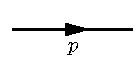
\includegraphics{prop}
	\end{center}
	
	We know that we will only have terms in $\Po$ of even powers of $\phi$.  Then for integer $n$, the term of order $j^{2 n}$ is proportional to
	\eq{
		\lam^n = \int \ddqxq \cdots \ddqxn \jxq \cdots \jxn \ev*{ T \phiq \cdots \phin }{0}
		= \int \ddqpf \abs{\jtp}^{2 n} \paren{ \frac{i}{p^2 - m^2 + i \eps} }^n.
	}
	So the whole perturbation series can be written as
	\eq{
		\Po = \abs{ 1 + \centergraphics{prop1} + \centergraphics{prop2} + \centergraphics{prop3} + \centergraphics{prop4} + \cdots }^2,
	}
	where each propagator represents one factor of $\lam$.  For the symmetry factor, there are $2^{2n / 2} = 2^n$ ways the $2n$ vertices can be chosen to be initial or final vertices, and a further $n!$ ways the $n$ initial vertices can be paired with the $n$ final vertices.  This gives us the symmetry factor $2^n n!$.  Then, using the power series~\cite{Exponential}
	\eq{
		e^x = \sumni \frac{x^n}{n!},
	}
	we can write
	\eq{
		\Po = \paren{ \sumni \frac{(-\lam)^n}{2^n n!} }^n
		= \paren{ \sumni \frac{1}{n!} \paren{ -\frac{\lam}{2} }^n }^n
		= ( e^{-\lam / 2} )^2
		= \ans{ e^{-\lam / 2} }
	}
	as desired. \qed
}



%\prob{}{
%	Compute the probability that the source creates one particle of momentum $k$.  Perform this computation first to $\order{j}$ and then to all orders, using the trick of \ref{4.1c} to sum the series.
%}



%\prob{}{
%	Show that the probability of producing $n$ particles is given by
%	\eq{
%		\Pn = \frac{\lam^n e^{-\lam}}{n!}.
%	}
%	This is a \emph{Poisson} distribution.
%}
%
%
%
%\prob{}{
%	Prove the following facts about the Poisson distribution:
%	\al{
%		\sumni \Pn &= 1, &
%		\evN &= \sumni n \Pn = \lam.
%	}
%	The first identity says that the $\Pn$s are properly normalized probabilities, while the second confirms our proposal for $\evN$.  Compute the mean square fluctuation $\ev{(N - \evN)^2}$.
%}






%\state{Decay of a scalar particle (Peskin \& Schroeder 4.2)}{
%	Consider the following Lagrangian, involving two real scalar fields $\Phi$ and $\phi$:
%	\eq{
%		\cL = \frac{1}{2} (\ptsm\Phi)^2 - \frac{1}{2} M^2 \Phi^2 + \frac{1}{2} (\ptsm\phi)^2 - \frac{1}{2} m^2 \phi^2 - \mu \Phi \phi \phi.
%	}
%	The last term is an interaction that allows a $\Phi$ particle to decay into two $\phi$s, provided that $M > 2m$.  Assuming that this condition is met, calculate the lifetime of the $\Phi$ to lowest order in $\mu$.
%}






%\state{Aspects of scaling behavior in QFT}{\hfix}

%\prob{}{
%	As discussed in class, massless free scalar field theory is invariant under scale transformations if we assign the appropriate scale dimension to the field $\phi$.  The action of dilations on coordinates is implemented by the operator $D = i \xm \ptsm$.  Find  the commutation relations of this operator with the operators that implement the Poincar\'{e} algebra of translations $\Psm = i \ptsm$ and Lorentz transformations $\Jsmn = i (\xsm \ptsn - \xsn \ptsm)$.  Find the canonical Noether current and Noether charge for this symmetry in the free field theory, and find the commutation relations of the charge with the field $\phi$ to show that it implements the infinitesimal form of the symmetry on the fields.  Check also that this current has the right commutation relations with the field theory Hamiltonian and momentum generators.
%}



%\prob{}{
%	The sound waves in a solid obey a wave equation, which at low enough wavelengths/energies is described by the action (for simplicity, consider one spatial dimension)
%	\eq{
%		\So = \int \ddtx (\ptst \phi \ptst \phi - \cs^2 \ptsx \phi \ptsx \phi)
%	}
%	where $\cs$ is the speed of sound in the material.  The field $\phi$ describes the distortion of the lattice away from equilibrium.  Model this situation by a lattice of atoms (mass $m$, lattice spacing $a$) interacting through harmonic nearest-neighbor forces (spring constant $k$).  Find the leading term in the action which corrects the above kinetic energy in a power series in $a \times (\text{derivatives})$ (this can be done for instance by expanding the exact dispersion relation for the chain of masses and springs).  Show that this correction term is an irrelevant perturbation of the action, so that all traces of the lattice structure disappear in the continuum limit $a \to 0$ (e.g.~all traces of the structure of interactions at the atomic level---such as a general potential $\Vr$ between the atoms rather than harmonic forces---disappear, being summarized in the constant $\cs$, and the effective action $\So$ is independent of the cutoff $a$).  Estimate the momentum scale at which the irrelevant corrections amount to 10\% of the total energy of a phonon.
%}


\makebib

\end{document}
